%% LyX 2.0.2 created this file.  For more info, see http://www.lyx.org/.
%% Do not edit unless you really know what you are doing.
\documentclass[a4paper,english]{article}
\usepackage[T1]{fontenc}
\usepackage[latin9]{inputenc}
\usepackage{babel}
\usepackage{array}
\usepackage{rotating}
\usepackage{multirow}
\usepackage{amsmath}
\usepackage{amssymb}
\usepackage{graphicx}
\usepackage[unicode=true]
 {hyperref}

\makeatletter

%%%%%%%%%%%%%%%%%%%%%%%%%%%%%% LyX specific LaTeX commands.
\pdfpageheight\paperheight
\pdfpagewidth\paperwidth

%% Because html converters don't know tabularnewline
\providecommand{\tabularnewline}{\\}

%%%%%%%%%%%%%%%%%%%%%%%%%%%%%% User specified LaTeX commands.
\usepackage{babel}
\usepackage{a4wide}

\@ifundefined{showcaptionsetup}{}{%
 \PassOptionsToPackage{caption=false}{subfig}}
\usepackage{subfig}
\makeatother

\begin{document}

\title{Modeling basic color term usage\\
with similarity-maximization games}


\author{Jos� Pedro Correia\\
(No. 10232095) MSc Logic \and Radek Ocel�k\\
(No. 10227709) MSc Logic}
\maketitle
\begin{abstract}
Basic color term usage in natural languages has seen a great deal
of research devoted to it in past decades. The reason is that the
topic has served as a kind of battleground for rival philosophical
standpoints regarding the nature of human language and cognition.

In this work, we explore the use of similarity-maximization signaling
games to model the evolution of color categories. The model combines
innate constraints in human color perception with cultural evolution
driven by the need for communicative success. To put the model to
a concrete test, we compare the outcome of our simulations directly
to real-world basic color term usage data collected in the World Color
Survey.

Although we do not find in our simulation results the same strong universal patterns that have been observed in natural languages, the level
of agreement between our simulation results and real-world languages
indicate that the model is on the right track to provide a good account
of how basic color term usage can develop within a community.
\end{abstract}

\section{The World Color Survey and the facts to be explained}

\label{sub:WCS-facts}

Berlin and Kay~\cite{Berlin69} pioneered a long tradition of research
into color term systems of world's languages. This broad typological
study pointed out that there clearly are universal tendencies concerning
repertoires of basic color terms in particular languages. The essential
claim for our purposes is an evolutionary one: there is a cross-linguistically
universal order in which color vocabularies are enriched by new terms.
The order of emergence is captured by the following implicational
hierarchy of universals: {[}white, black{]} $<$ {[}red{]} $<$ {[}green,
yellow{]} $<$ {[}blue{]} $<$ {[}brown{]} $<$ {[}purple, pink, orange,
gray{]}

This hierarchy expresses a complex constraint which was claimed to
apply to all existing natural languages. It should be read as follows:
if a language has a well-established term for red (that is, a term
covering the point of the color space which is the prototypical denotation
of the English ``red''), it also has basic terms for white and for
black, but not necessarily \textit{vice versa}. Similarly, if it has
one for green or for yellow, it also has one for red, and so on. According
to this picture, color term systems are far from being relativistically
arbitrary: whatever number of terms they contain, these terms can
carve the color space only in certain ways. For example, in a language
with three color terms, these are bound to cover, respectively, red,
black, and white. The English terms are in fact misleading, since
each language is supposed to fully partition the color space. In the
last case, the term for red is likely to cover violet or orange as
well and the other two terms would rather correspond to ``dark''
and ``light''.

In order to examine the main theses of the founding study, the World
Color Survey (WCS)~\cite{WCS} was conducted in the subsequent decades.
It substantially broadened the empirical base and improved the methodology
of the previous work, performing field research for 110 unwritten
languages (listed by Regier, Kay and Cook~\cite{Reg05}) with a negligible
level of genetic interrelatedness, with 24 informants per language
on average (cf.\ Kay and Cook~\cite{KayEnc} for methodology). The
employed color system was one of 330 Munsell chips, 320 of them in
the Lenneberg and Roberts array of 40 hue columns and 8 levels of
lightness, at maximum saturation, plus an achromatic column of 10
chips from white to black.

The results of the WCS concerning the universality of color terms
emergence are described by Kay and Maffi~\cite{Kay99}. In their
work, the empirically documented color term systems are classified
into 9 types spread over 5 stages with respect to how six focal points
of the color space, corresponding to prototypical denotations of English
``white''~(W), ``red''~(R), ``yellow''~(Y), ``green''~(G),
``blue''~(Bu), ``black''~(Bk), are grouped by the vocabulary
of each particular language%
\footnote{Some formulations by Kay and Maffi~\cite{Kay99} are misleading,
but Kay et al.~\cite{Kay97} make it clear that what is considered
are only partitions of the six focal points, regardless of possible
color terms that do not pick any of them. So, e.g., a term covering
only purple is not considered ``basic'' in this context; this follows
from the assumption of psychophysiological centrality of the six considered
colors. Consequently, a language with more than 4 color terms still
belongs to Stage III, if these terms split the 6 focal points into
just 4 groups.%
}. For instance, in Stage II (languages with 3 basic color terms) there
is only one observed type, {[}W; R+Y; Bk+G+Bu{]}%
\footnote{This notation indicates that the language has one color term that
encompasses the prototypical denotation of ``white'' in English,
another that encompasses ``red'' and ``yellow'', and another that
encompasses ``black'', ``green'', and ``blue''.%
}; in Stage III (4 basic color terms) there are the types {[}W; R;
Y; Bk+G+Bu{]}, {[}W, R+Y, G+Bu, Bk{]} and {[}W, R, Y+G+Bu; Bk{]}.
The authors note that there are five possible evolutionary trajectories
between stages I to V, assuming that any evolutionary step consists
in splitting the denotation (the covered focal points) of one term
of the previous system in two. The trajectory {[}W+R+Y; Bk+G+Bu{]}
$>$ {[}W, R+Y, Bk+G+Bu{]} $>$ {[}W, R+Y, G+Bu, Bk{]} $>$ {[}W;
R; Y; G+Bu; Bk{]} $>$ {[}W; R; Y; G; Bu; Bk{]} is the most represented
one in the WCS, capturing 91 of the 110 languages.

The way the empirical results are presented requires some discussion.
The talk of evolutionary paths as instantiated by the languages is
slightly misleading: what was really observed was in each case a snapshot
of a color term system belonging to one of the 9 types, or to a transition
between two of them. These observed transitions are the maximum of
diachrony captured in the WCS; apart from this we cannot infer anything
about how a particular observed color vocabulary actually came about.
This having been clarified, the formulation in terms of these emergence
trajectories and the representation of the particular types seems
more appropriate than the original strong formulation in terms of
implicational hierarchy. First, it draws attention to the almost universal%
\footnote{Rare exceptions are discussed in section 3 of Kay and Maffi \cite{Kay99}.%
} principle of partitioning the color space by the available terms,
and consequently to the fact that if a color vocabulary is enriched
with an additional term, the denotation of some or all of the already
established terms is likely to be modified. Second, the gathered data
do not seem univocal enough to formulate an implicational hierarchy
as strong as that of Berlin and Kay~\cite{Berlin69}, and anyway,
in order to formulate any such generalization, the data would have
to be statistically evaluated with this in mind. Admittedly, an overall
quantitative evaluation of the WCS data has been done by Kay and Regier~\cite{Kay03}
and Regier, Kay and Cook~\cite{Reg05}, and it has shown a clear
non-random match among color term systems of world's languages, thus
refuting the position of full relativism in this respect. But whether
\textit{particular} generalizations (implicative or other) are valid
is an altogether different question. We conjecture that a consequential
part of the original hierarchy would not find a significant support
in the data, since in the sample there are relatively little languages
spread among the types with 4 or less basic color terms, as opposed to about
80 languages with 5 or 6 basic color terms or in between.

In the general lack of statistically conclusive support for individual
universal features of human color categorization, we will focus on
the two of them that can be most reliably inferred from the absolute
numbers reported by Kay and Maffi~\cite{Kay99}. One is that vocabularies
with 3 basic color terms tend to partition the color space according
to the scheme {[}W; R+Y; Bk+G+Bu{]}, that is, to separate the warm
colors while keeping the cool colors together with black. This is
the only reported type for Stage II, instantiated by 6 languages.
The other universal feature to focus on is the evolutionarily late
division of green and blue: {[}W; R; Y, G+Bu; Bk{]} is by far the
most represented type of systems with 5 basic terms (Stage IV), instantiated
by 41 languages. The strong universal tendencies to carve up the color
space in the described way when, respectively, three and five basic
color terms are present, will be in the following regarded as the
strongest, best substantiated empirical facts to be explained.




\section{Related work}

The general debate on the nature of cognitive categories is dominated
by three competing paradigms, nativism, empiricism and culturalism,
the third often presented as a solution to the aged dilemma between
the first two (cf. Steels and Belpaeme~\cite{Steels05} and their
references). The debate on color categorization, specifically, is
furthermore structured along the dimension of universality vs.\ relativity,
which is arguably a distinct one, despite affinities such as that
between nativism and universalism. The WCS has posed this question
as straightforwardly empirical and provided data; as a result, recent
positions on both the universalist~\cite{Kay03,Reg05} and the relativist~\cite{Rob05}
side are rather moderate.

Granted that there \textit{are} universal tendencies in color categorization,
explanation of these (and of the remaining relativity) has been approached
in several ways. Kay and Maffi~\cite{Kay99} themselves present an
updated version of a model that had been continuously developed by
the WCS authors, on the (close to) nativist assumption of 6 naturally
focal colors. The issue has been also studied within the broadly culturalist
framework of the Iterated Learning Model~\cite{Smith03,Dowm07}.
However, here we will only discuss in detail the approaches that directly
motivate our own model, in which the emergence of categories is conceived
in terms of cultural interaction on the basis of innate characteristics
of human perception. In a nutshell, these are works by Baronchelli
et al.~\cite{Baron10} and by Loreto et al.~\cite{Lor12}, focusing
on the impact of perceptual constraints on routinized cultural interaction;
the more recent work of the WCS authors~\cite{Reg07} investigating
partitions of the perceptual space in terms of optimality; and J�ger
and van Rooij's~\cite{Rooij07} proposal to treat the issue in game-theoretical
terms. 

The first two of our motivating approaches jointly assume that universality
of categorization might be explainable in terms of specific characteristics
of human visual perception. We first discuss the work by Baronchelli
et al.~\cite{Baron10} and Loreto et al.~\cite{Lor12}, who attempt
to derive the universals from a particular formulation of the dependence
of perception on the physical character of the input. We then outline
the explanatory strategy of Regier, Kay and Khetarpal~\cite{Reg07},
which appears to be a more general, though in a sense less elaborated,
version of the former.


\subsection{Just Noticeable Difference}

Baronchelli et al.~\cite{Baron10}, as well as Loreto et al.~\cite{Lor12},
appeal in explanation to a simple characteristic of human visual perception,
called Just Noticeable Difference (JND). The human JND is a psychophysiologically
determined function which for any given wavelength from the extent
of the visible spectrum gives the minimal difference in wavelength
of two hues that are distinguishable by the human eye in that particular
region of the spectrum. This function is implemented as a constraint
on cultural interaction of artificial agents, conceived roughly along
the lines of Steels and Belpaeme's ``culturalist model''~\cite{Steels05}.
In this setting, color term vocabularies and categorical systems of
individual agents in a population are made to co-evolve through their
repetitive participation in standardized linguistic interaction over
empirical input (``the Category Game''). Similarity between the
emergent systems and those observed empirically is then supposed to
vindicate the explanatory role of the human JND.

Despite general formulations (``excellent quantitative agreement''
with the WCS data), Baronchelli et al.\ are successful only in a
specific sense. Their simulation does not demonstrate for particular
universal features of human color categorization how these might have
been arrived at. It shows only that categorical systems developed
via cultural interaction constrained by the human JND are less dispersed
across populations than when a flat, non-human JND is used. The only
quantitative agreement, then, is between the ratio of the two respective
values of dispersion, and the dispersion ratio of the actually observed
categorical systems of the WCS, compared to a specific randomization
of these (as done by Kay and Regier~\cite{Kay03}). The agreement
of these two ratios on approximately 1.14 is remarkable, but hard
to interpret in isolation. %both these values are construed in such a complicated fashion that proper interpretation of the match can hardly be straightforward. RO: I insist upon this, though it may not sound as a correct argument. The thing is that evolution in silica, according to a specific dynamic, is something quite different and trasparent in comparison with the overall evolution of world's languages with the immense number of participating factors (including genetic relations, language contact, wars and whatever). While in some respects the artificial dynamic may be almost reasonable model for the latter, I'm pretty sure that from an out-of-the-blue coincidence of two similarly constructed numbers describing outcomes of these two processes absolutely nothing can be inferred.


Loreto et al.~\cite{Lor12} come somewhat closer to explanation of
particular universals of color categorization. The human JND as a
constraint on routine language interaction over empirical input is
sufficient for them to derive a hierarchy of color terms according
to the time it takes for color terms in various regions of the visible
spectrum to be agreed upon within the population. The claim about
''excellent quantitative agreement with the empirical observations
of the WCS'' is not further substantiated in the paper. But the authors
rightly point out that their hierarchy, {[}red, (magenta)-red{]} $<$
{[}violet{]} $<$ {[}green/yellow{]} $<$ {[}blue{]} $<$ {[}orange{]}
$<$ {[}cyan{]}, is similar to the implicational hierarchy of Berlin
and Kay \cite{Berlin69}. Let us discuss the relevance of this finding.

First, there seems to be a methodological problem with choice of color
terms and their matching to regions of the spectrum. This should,
arguably, have been done either by selecting a set of cross-linguistically
basic colors and locating them in the spectrum, or by selecting important
points or sections of the JND function and reading off the respective
colors; but an opaque combination of both seems to have taken place.
In the first case we would expect both green and yellow in the selection,
instead of green/yellow, and we might challenge the inclusion of cyan
and (magenta)-red. In the second case, while most of the selected
points reflect peaks and valleys of the function, (magenta)-red does
not, violet and red are disputable, and there is an unreflected valley
between violet and blue. Some of this could be actually resolved in
favor of the parallel between the achieved hierarchy and Berlin and
Kay's hierarchy; first of all, there are reasons to pick only red
for the experiment, instead of red, (magenta)-red and violet. But
there remains the problem that green/yellow in the achieved hierarchy
is a single transitional color, while in Berlin and Kay's hierarchy
green and yellow are two distinct colors occupying the same position.

Moreover, let us remember that the work by Berlin and Kay~\cite{Berlin69}
is a dated reference and there is little point in evaluating explanatory
proposals concerning universals of color categorization against the
hierarchy stated there, in presence of the WCS data, the superiority
of which is both empirical and methodological. Our discussion in Section~\ref{sub:WCS-facts}
indicate that the mismatch between the actual findings by Loreto et
al.~\cite{Lor12} and the cross-linguistic reality would have been
magnified by an up-to-date evaluation, rather than attenuated. While
we believe that the features of human perception that are captured
by the JND function should play an important explanatory role regarding
linguistic universals, we believe a more up-to-date investigation
is still necessary.


\subsection{The CIELAB space}

The previous approach appeals to a particular feature of human perception
(the resolution power in different frequencies of visible light).
The explanatory strategy adopted by Regier, Kay and Khetarpal~\cite{Reg07},
with reference to Jameson and D'Andrade~\cite{Jam97}, is a more
general version of that. Instead of carving up a physically defined
space (one-dimensional in the previous case), they consider partitions
of the psychologically relevant, 3D color space CIELAB. This color
space is designed so that standard Euclidean distance of two hues
corresponds to their psychological dissimilarity. By using this color
space, the constraint on human color perception embodied by the JND
is encompassed rather than discarded as a source of explanation, for
what it expresses has to be involved also in construction of any psychologically
relevant space. When the Munsell color palette used in the WCS is
projected into the CIELAB space, its chips mark the surface of an
irregular sphere. What is then discussed are partitions of the set
of color points thus arranged. The authors convincingly show a strong
preference of the WCS languages for efficient partitions, efficient
in terms of maximizing the compactness of their color categories in
the CIELAB space. What this means is that the closer two chips are
in the perceptual space, the more likely they will be lumped under
the same color term.

This is clearly an important result, pointing to optimality as an
essential factor of color categorization. However, this line can be
drawn further. Given the specific way of evaluation (each language's
actual partition vs.\ its various rotations around the sphere), the
results cannot directly account for any particular linguistic universal
in question. For instance, we do not see whether the most efficient
ways of partitioning the figure into 5 regions involve keeping blue
and green together. Another issue is that optimality or efficiency
is a static feature of a categorical system (of an individual speaker
or of a language \textit{in abstracto}), without it being clear how
it might have come about. In our approach we adopt the idea of the
overall character of human visual perception, reflected in the CIELAB
color space, as the likely source of universals of color categorization.
For sake of comparability with the WCS data we also work with the
projected Munsell palette. However, the optimization strategy used
by Regier et al.~\cite{Reg07} to calculate partitions of the color
space has no realistic underlying motivation. Therefore we are interested
in investigating an evolutionary, agent-based dynamic of cultural
interaction, as in the game-theoretic formulation proposed by J�ger
and van Rooij~\cite{Rooij07}.


\subsection{Similarity-maximization games}

J�ger and van Rooij~\cite{Rooij07} construe the problem as a similarity-maximization
signaling game. Nature picks a point from the color space as the meaning
to be conveyed; the sender sends one term from a finite set to signal
the chosen meaning to the receiver; the receiver interprets the received
signal by choosing a point from the color space. The payoff this signaling
action brings to both the sender and the receiver is a monotonically
decreasing function of the distance in the color space between the
receiver's interpretation and the speaker's intended meaning. In general,
the sender strategy is a function from the set of points of the color
space to (a probabilistic distribution over) the given set of terms,
and the receiver strategy is a function from the set of terms to (a
probabilistic distribution over) the set of points of the color space.
If we let the game be played repetitively and relate payoffs from
each particular game to the ''fitness'' of the sender and the receiver
strategy employed in that game, or the probability that they will
be employed in the next run, we get an evolutionary process with a
specific dynamic. This process can be, in principle, viewed as a model
of evolution of color categories in a community. How various parameters
of such a model are to be set up is, of course, subject to discussion.

We chose to base our evolutionary model in similarity-maximization
signaling games, rather than in the Category Game of Steels and Belpaeme~\cite{Steels05},
adopted by Baronchelli et al.~\cite{Baron10} and Loreto et al.~\cite{Lor12}.
In the former setting, categories are inherently linguistic and can
be unproblematically called ''concepts'' as well. The latter approach,
on the other hand, makes the conceptual distinction between perceptual
and linguistic categories. Each agent, based on empirical input, individually
divides a continuous perceptual space into regions (perceptual categories)
within which she cannot further distinguish. A linguistic category
then emerges through subsuming of adjacent perceptual categories under
a single term. As perceptual categorization independent of language
seems to be a problematic notion to us, we prefer the simpler formulation
in terms of signaling games. Admittedly, we consider only the 330
Munsell chips as the color space, instead of the continuous space.
This choice is motivated by simplicity, especially for allowing a
more direct evaluation against the WCS data, but it can be seen as
a preliminary perceptual categorization of the continuous space. However,
a difference is that in our case the perceptual space is not carved
up arbitrarily by individual agents, but uniformly and in roughly
homogeneous way with respect to human resolution abilities.


\section{Methodology}

As described above, We model the evolution of color terms as a similarity-maximization
signaling game, in the spirit of J�ger and van Rooij~\cite{Rooij07}.
We make, however, a number of changes to better fit the problem at
hand. Quantitative evaluation is performed against the WCS data by
matching simulation results with actual languages and calculating
the quality of the match.


\subsection{Simulation setup}

\label{sub:simulation}

First of all, we use Munsell chips as individual percepts and define
their distance in terms of their coordinates in CIELAB color space,
as is done by Regier et al.~\cite{Reg07}. The perceptual space to
be used in the game consists therefore of 330 points which can be
indexed by hue (levels from 0 to 40) and value (10 levels for the
achromatic chips, 8 for the others) or by coordinates in CIELAB space
$L$, $a$, $b$. We used the mapping from hue and value to CIELAB
space provided with the WCS data%
\footnote{Obtained from \href{http://www1.icsi.berkeley.edu/wcs/data/cnum-maps/cnum-vhcm-lab-new.txt}{http://www1.icsi.berkeley.edu/wcs/data/cnum-maps/cnum-vhcm-lab-new.txt}
(accessed 17/01/2013).%
}. Given two points and their CIELAB coordinates $x_{1}=\left\langle L_{1},a_{1},b_{1}\right\rangle $
and $x_{2}=\left\langle L_{2},a_{2},b_{2}\right\rangle $, their similarity
is given by: 
\[
sim\left(x_{1},x_{2}\right)=e^{-c\times\left(dist\left(x_{1},x_{2}\right)\right)^{2}}
\]
 where $dist\left(x_{1},x_{2}\right)$ is the euclidean distance in
CIELAB space: 
\[
dist\left(x_{1},x_{2}\right)=\sqrt{\left(L_{1}-L_{2}\right)^{2}+\left(a_{1}-a_{2}\right)^{2}+\left(b_{1}-b_{2}\right)^{2}}
\]
 To be in line with Regier et al.~\cite{Reg07} we use $c=0.001$
for all simulations.

The similarity-maximization game consists of the tuple $\left\langle T,\Pr,M,U\right\rangle $,
where $T$ is the perceptual space described above, $\Pr\in\Delta\left(T\right)$
is a probability distribution over $T$, $M$ is the set of messages
available, and $U\in T\times T\rightarrow\mathbb{R}$ is the utility
function for both speaker and hearer. We define only one utility function
for both speaker and hearer, thus we assume perfectly cooperative
interests. Furthermore, we assume that talk is cheap and utility is
directly proportional to similarity, \emph{i.e.}\ $U\left(x_{1},x_{2}\right)=sim\left(x_{1},x_{2}\right)$.
We used a uniform $\Pr$ in all simulations, but we include it in
the formulation of the model to not deviate from J�ger and van Rooij~\cite{Rooij07}
and because we will come back to it in Section~\ref{sec:discussion}.

Regarding game dynamics, we used the replicator equation over mixed
strategies. A sender strategy $\sigma\in T\rightarrow\Delta\left(M\right)$
associates to each point in the perceptual space a probability distribution
over the set of messages. A receiver strategy $\rho\in M\rightarrow\Delta\left(T\right)$
associates to each message a probability distribution over all points
in perceptual space. Probability values should be interpreted as percentages
of a hypothetical population. Therefore, if $\sigma\left(x_{1},m_{1}\right)=0.7$,
this should be interpreted as ``$70\%$ of the population uses message
$m_{1}$ when observing point $x_{1}$''. The dynamics update these
strategies according to their expected utility. The state of each
strategy at time instant $t+1$ is defined as follows: 
\[
\sigma_{t+1}\left(x,m\right)=\sigma_{t}\left(x,m\right)\times\frac{\textnormal{EU}_{\sigma_{t}}\left(m\mid x,\rho_{t}\right)\times\left|M\right|}{\underset{m^{\prime}\in M}{\sum}\textnormal{EU}_{\sigma_{t}}\left(m^{\prime}\mid x,\rho_{t}\right)}
\]
 
\[
\rho_{t+1}\left(m,x\right)=\rho_{t}\left(m,x\right)\times\frac{\textnormal{EU}_{\rho_{t}}\left(x\mid m,\sigma_{t}\right)\times\left|T\right|}{\underset{x^{\prime}\in T}{\sum}\textnormal{EU}_{\rho_{t}}\left(x^{\prime}\mid m,\sigma_{t}\right)}
\]
 where expected utilities are defined as: 
\[
\textnormal{EU}_{\sigma}\left(m\mid x,\rho\right)=\underset{x^{\prime}\in T}{\sum}\rho\left(x^{\prime}\mid m\right)\times U\left(x,x^{\prime}\right)
\]
 
\[
\textnormal{EU}_{\rho}\left(x\mid m,\sigma\right)=\underset{x^{\prime}\in T}{\sum}\Pr\left(x^{\prime}\right)\times\sigma\left(m\mid x^{\prime}\right)\times U\left(x^{\prime},x\right)
\]
 Starting conditions $\sigma_{0}$ and $\rho_{0}$ are initialized
with random values for every simulation. All simulations were ran
until a convergence criterion was met. The criterion was that the
total absolute change in both sender and receiver strategy was under
$1\%$, \emph{i.e.}: 
\begin{eqnarray*}
 & \underset{x\in T}{\sum}\underset{m\in M}{\sum}\left|\sigma_{t+1}\left(x,m\right)-\sigma_{t}\left(x,m\right)\right|<0.01\\
 & \wedge\\
 & \underset{m\in M}{\sum}\underset{x\in T}{\sum}\left|\rho_{t+1}\left(m,x\right)-\rho_{t}\left(m,x\right)\right|<0.01
\end{eqnarray*}



\subsection{Quantitative evaluation}

\label{sub:quantitative-evaluation}

Following the approach by Regier et al.~\cite{Reg07}, we calculated
a mode map per language in the WCS data. Each language was then classified
regarding the number of main color terms. Since Regier et al.\ did
not provide a clear criterion for what they consider a main color
term, we employed our own heuristic: we counted for each language
how many color terms cover at least $5\%$ of the space, \emph{i.e.}\ at
least $16$ Munsell chips.

We can then try to match two $n$-term languages (or simulation results)
$L_{1}$ and $L_{2}$ by mapping terms in one language to terms in
the other. The procedure was to establish the mapping based on the
amount of overlap between terms as follows: 
\begin{enumerate}
\item Calculate, for each pair of terms $t_{1}\in L_{1}$ and $t_{2}\in L_{2}$,
the number of chips they have in common; 
\item Establish a one-to-one mapping starting with the two terms that have
the highest overlap until no more terms are left or no overlap exists
between the remaining terms. 
\end{enumerate}
The quality of each pairing can be calculated in terms of precision
and recall, \emph{i.e.}\ what percentage of $t_{1}$ chips are also
$t_{2}$ and what percentage of $t_{2}$ chips are also $t_{1}$.
The overall quality of the mapping can be calculated in terms of accuracy,
\emph{i.e.}\ what percentage of total overlap is there with the established
mapping.

The accuracy numbers can then be summarized to give an impression
of the overall match between our languages (or simulation results)
and the languages in the WCS. As reference points for comparison we
calculated these numbers not only for our simulation results but for
three other scenarios, namely: 
\begin{enumerate}
\item Matching each WCS language against its peers (in number of main color
terms). This establishes a pragmatic upper bound to how well we can
expect a simulation to be able to perform; 
\item Simulation results performed with a neutral similarity metric. Since
the Munsell chips are distributed in CIELAB space as an irregular sphere,
for these results we laid them out as a regular sphere. For that we
used as spherical coordinates, value to indicate the elevation angle,
hue to indicate the azimuth angle, and a fixed radius estimated from
the irregular sphere. Distance was then computed by converting these
coordinates to Cartesian coordinates and calculating the Euclidean
distance; 
\item Random assignment of color terms to chips (basically the initial conditions
of the simulation). This establishes a lower bound for comparison.
%note on why the results are better than 1/n?

\end{enumerate}

\section{Results}

As described in Section~\ref{sub:quantitative-evaluation}, all languages
in the WCS were classified in terms of their number of main color
terms. The following table summarizes the results:

\begin{center}
\begin{tabular}{r|rrrrrr}
Number of main color terms  & 3  & 4  & 5  & 6  & 7  & 8\tabularnewline
\hline 
Number of languages  & 6  & 12  & 31  & 40  & 14  & 7 \tabularnewline
\end{tabular}
\par\end{center}

\noindent Based on these results, we ran $10$ simulations for each
of these categories.


\subsection{Specific evaluation of the evolutionary predictions}

To evaluate the model against the two particular facts concerning
the evolutionary order of color terms emphasized in Section~\ref{sub:WCS-facts},
we classified the resulting categorical systems of $60$ simulations
into types spread over stages, as done by Kay and Maffi~\cite{Kay99}.
Analogically to their work, the classification was based on the way
in which the resulting systems partitioned the $6$ assumed focal
color points. After Kay~\cite{Kay05}, we took the focal points to
be represented by the following chips: A0 for white, C9 for yellow,
G1 for red, F17 for green, F29 for blue, and J0 for black. On the
whole, there is little resemblance between our outcome and the empirical
classification of Kay and Maffi~\cite{Kay99}. Most of our Stage
II is covered by the types {[}W+Y; R+Bu; G+Bk{]} and {[}W+Y; G+Bu;
R+Bk{]}, whereas the only type attested in the WCS, {[}W; R+Y; Bk+G+Bu{]},
is not represented in our Stage II. In our stage IV, the most represented
types are {[}W; Y+Bk; G; Bu; R{]}, {[}W; Y; G; R+Bu; Bk{]} and {[}W;
Y; R; G+Bk; Bu{]}. The type {[}W; R; Y, G+Bu; Bk{]}, which is dominant
among the WCS languages of Stage IV, is lacking in our results.

It is nonetheless important to note that the reported numbers crucially
depend on the considered position of the focal points, and that a
slight change in this respect can substantially modify the resulting
picture. The position of focal blue is a most striking example. In
our classification there are $19$ systems in which focal blue and
red are subsumed under a common term. However, if we regarded the
chip F28 instead of the neighbouring F29 as the focal blue, $17$
of them would have to be reclassified, almost exclusively in favour
of types in which focal blue is lumped together with focal green,
or with focal green and focal black. That would bring our results
a little bit closer to the findings of Kay and Maffi~\cite{Kay99}.
Since we do not see independent theoretical motivation for moving
the focal points in this or another particular way, we do not follow
this line further. It is worth attention, though, especially as it
is not clear whether Kay and Maffi~\cite{Kay99} based their classification
on a set of focal points identical to ours. Table~\ref{tab:stages}
shows the representation of types in stages, assuming the basic set
of focal points, and after the minimal change to focal blue, as well as
the numbers reported by Kay and Maffi~\cite{Kay99}.

\begin{table}
\begin{centering}
\begin{tabular}{rrrrl}
\hline 
Type & Basic & Focal blue $\rightarrow$ F28 & Kay and Maffi~\cite{Kay99} & \tabularnewline
\hline 
W+Y; R+Bu; G+Bk & 6 & 1 & - & \multirow{5}{*}{Stage II}\tabularnewline
W+Y; R+Bk; G+Bu & 4 & 4 & - & \tabularnewline
W+Y; R; G+Bu+Bk & 2 & 5 & - & \tabularnewline
W+Bu; R+Y+Bk; G & 1 & - & - & \tabularnewline
W; R+Y+Bk; G+Bu & - & 1 & - & \tabularnewline
W; R+Y; G+Bu+Bk & - & - & 6 (+4) & \tabularnewline
\hline 
W; R+Bu; Y; G+Bk & 4 & 1 & - & \multirow{10}{*}{Stage III}\tabularnewline
W+Y; R+Bu; G; Bk & 3 & - & - & \tabularnewline
W; R+Bu; Y+Bk; G & 2 & - & - & \tabularnewline
W; R; Y+Bk; G+Bu & 2 & 6 & - & \tabularnewline
W+Y; R; G+Bk; Bu & 2 & 4 & - & \tabularnewline
W+Y; R+Bk; G; Bu & 1 & 1 & - & \tabularnewline
W; R+Y; G+Bu; Bk & - & 1 & 3 (+7) & \tabularnewline
W+Y; R; G+Bu; Bk & - & 2 & - & \tabularnewline
W; R; Y; G+Bu+Bk & - & 2 & (+8) & \tabularnewline
W; R+Bk; Y; G+Bu & - & 1 & - & \tabularnewline
W; R; Y+G+Bu; Bk & - & - & 2 (+2) & \tabularnewline
\hline 
W; R; Y+Bk; G; Bu & 5 & 3 & - & \multirow{8}{*}{Stage IV}\tabularnewline
W; R+Bu; Y; G; Bk & 4 & - & - & \tabularnewline
W; R; Y; G+Bk; Bu & 4 & 6 & - & \tabularnewline
W; R; Y; G; Bu+Bk & 2 & 3 & 3 (+2) & \tabularnewline
W; R+Y; G; Bu; Bk & 2 & 1 & - & \tabularnewline
W+Y, R; G; Bu; Bk & 1 & 2 & - & \tabularnewline
W; R+Bk; Y; G; Bu & 1 & - & - & \tabularnewline
W; R; Y; G+Bu; Bk & - & 4 & 41 (+16) & \tabularnewline
W; R; Y+G; Bu; Bk & - & - & 1 & \tabularnewline
\hline 
W; R; Y; G; Bk; Bu & 14 & 12 & 23 (+15) & \multirow{1}{*}{Stage V}\tabularnewline
\hline 
\end{tabular}
\par\end{centering}

\caption{Classification of simulations into types in terms of how they partition the 6
focal points, with the basic set of points and with focal blue changed
from F29 to F28. For comparison, we include also the numbers reported by Kay and Maffi~\cite{Kay99}
for the languages in the WCS. Numbers between parenthesis correspond to languages that
are either in transition to or from a certain type, or are considered a mix of that type and another one.}


\label{tab:stages} 
\end{table}


In the following, we evaluate our model as to its general predictive
power with respect to the documented languages of the WCS. In this
part of evaluation, all 330 chips are treated equally and the question
of focal colors plays no role.


\subsection{General quantitative evaluation}

We established mappings between each of the $60$ outcomes of the
simulations and the languages in the WCS in the respective categories.
For example, for $4$ terms we have $10$ simulations matched against
$12$ languages, thus $120$ accuracy values. Table~\ref{tab:overall-statistics}
contains the overall statistics for each category ($n$ is the number
of terms) in each scenario. We illustrate these numbers in Figure~\ref{fig:plots}
with the simulations involved in the best and worst matches.

\begin{table}
\begin{centering}
\begin{tabular}{rrrrrrrl}
\hline 
$n$  & Min.  & 1st Qu.  & Median  & Mean  & 3rd Qu.  & Max.  & \tabularnewline
\hline 
3  & 0.779  & 0.833  & 0.870  & 0.865  & 0.909  & 0.930  & \multirow{6}{*}{\begin{sideways}
WCS
\end{sideways}}\tabularnewline
4  & 0.336  & 0.545  & 0.630  & 0.629  & 0.712  & 0.836  & \tabularnewline
5  & 0.373  & 0.603  & 0.700  & 0.688  & 0.776  & 0.900  & \tabularnewline
6  & 0.400  & 0.606  & 0.679  & 0.670  & 0.739  & 0.879  & \tabularnewline
7  & 0.379  & 0.521  & 0.588  & 0.600  & 0.673  & 0.818  & \tabularnewline
8  & 0.488  & 0.600  & 0.715  & 0.690  & 0.741  & 0.888  & \tabularnewline
\hline 
3  & 0.394  & 0.468  & 0.602  & 0.583  & 0.692  & 0.788  & \multirow{6}{*}{\begin{sideways}
simulations
\end{sideways}}\tabularnewline
4  & 0.324  & 0.479  & 0.552  & 0.547  & 0.606  & 0.761  & \tabularnewline
5  & 0.388  & 0.500  & 0.533  & 0.542  & 0.573  & 0.703  & \tabularnewline
6  & 0.364  & 0.455  & 0.497  & 0.501  & 0.545  & 0.661  & \tabularnewline
7  & 0.376  & 0.458  & 0.486  & 0.489  & 0.521  & 0.630  & \tabularnewline
8  & 0.361  & 0.447  & 0.476  & 0.492  & 0.548  & 0.664  & \tabularnewline
\hline 
3  & 0.421  & 0.533  & 0.579  & 0.573  & 0.618  & 0.703  & \multirow{6}{*}{\begin{sideways}
perfect sphere
\end{sideways}}\tabularnewline
4  & 0.324  & 0.412  & 0.458  & 0.457  & 0.495  & 0.591  & \tabularnewline
5  & 0.261  & 0.400  & 0.452  & 0.447  & 0.486  & 0.600  & \tabularnewline
6  & 0.285  & 0.412  & 0.442  & 0.441  & 0.476  & 0.573  & \tabularnewline
7  & 0.318  & 0.418  & 0.448  & 0.444  & 0.473  & 0.570  & \tabularnewline
8  & 0.327  & 0.405  & 0.427  & 0.425  & 0.447  & 0.509  & \tabularnewline
\hline 
3  & 0.321  & 0.342  & 0.348  & 0.350  & 0.355  & 0.379  & \multirow{6}{*}{\begin{sideways}
random
\end{sideways}}\tabularnewline
4  & 0.224  & 0.270  & 0.285  & 0.282  & 0.294  & 0.321  & \tabularnewline
5  & 0.182  & 0.224  & 0.233  & 0.234  & 0.245  & 0.270  & \tabularnewline
6  & 0.164  & 0.203  & 0.212  & 0.214  & 0.224  & 0.258  & \tabularnewline
7  & 0.155  & 0.179  & 0.191  & 0.190  & 0.200  & 0.239  & \tabularnewline
8  & 0.148  & 0.170  & 0.179  & 0.179  & 0.188  & 0.221  & \tabularnewline
\hline 
\end{tabular}
\par\end{centering}

\caption{Summary statistics of match accuracy against languages in the WCS.}


\label{tab:overall-statistics} 
\end{table}


\begin{figure}
\subfloat[Simulation with one of the best average accuracy values: 0.715. Best
match against Kwerba (Figure~\ref{fig:kwerba}). Worst match against
Nafaanra (Figure~\ref{fig:nafaanra}).]{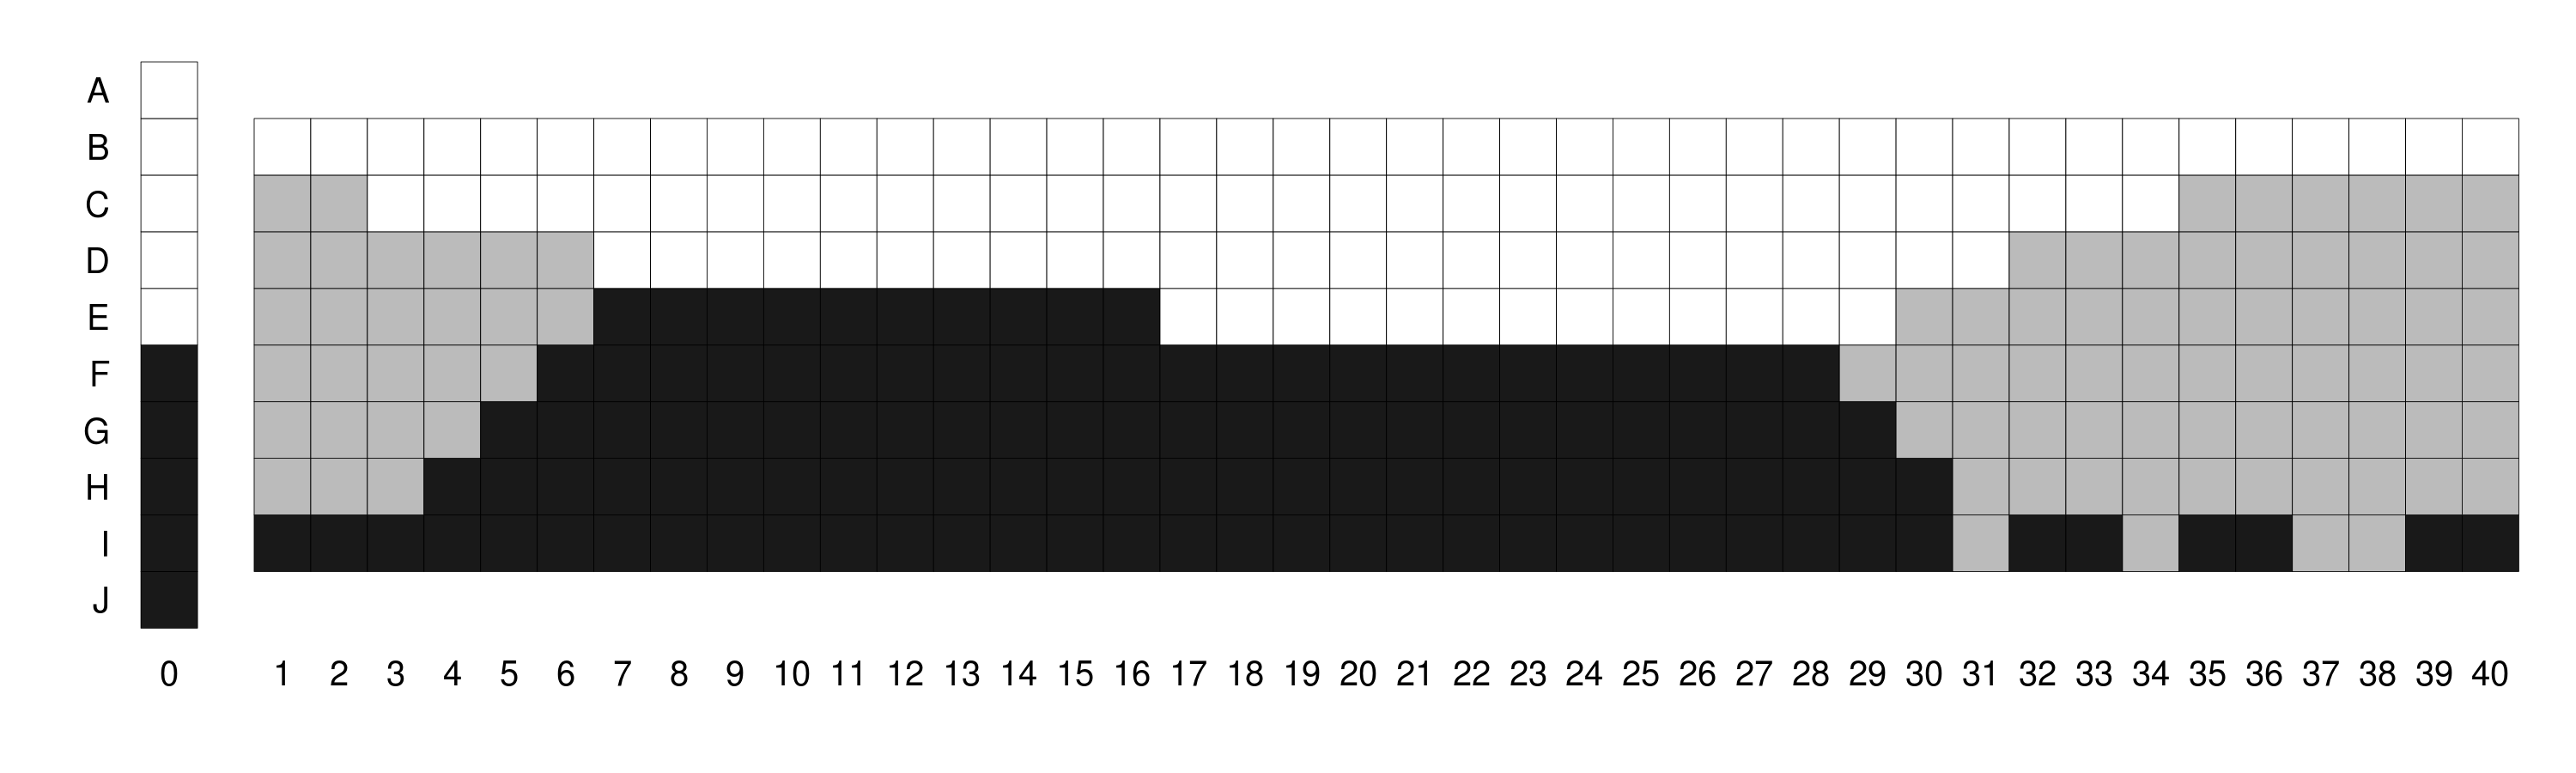
\includegraphics[width=0.48\textwidth]{3-2}

\label{fig:best-simulation}

}\hfill{}\subfloat[Simulation with one of the worst average accuracy values: 0.449. Best
match against Ch�cobo (Figure~\ref{fig:chacobo}). Worst match against
Culina (Figure~\ref{fig:culina}).]{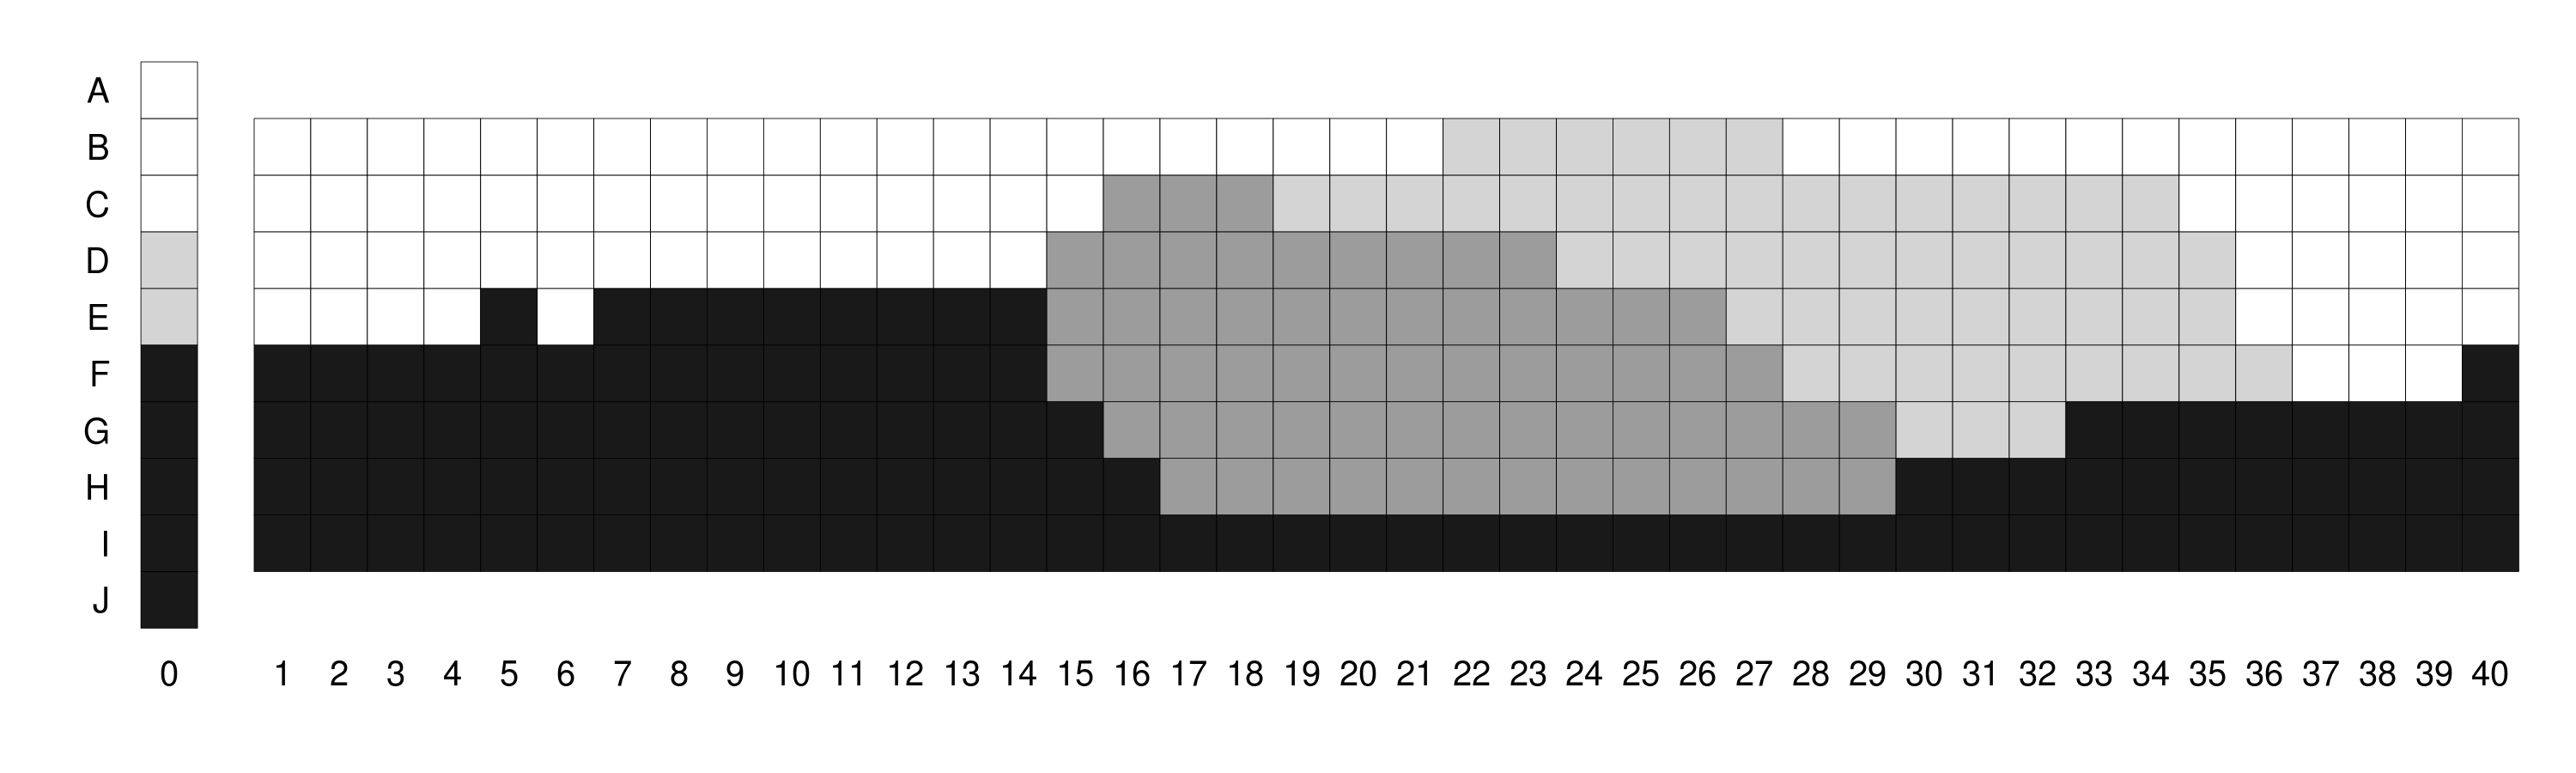
\includegraphics[width=0.48\columnwidth]{4-2}

\label{fig:worst-simulation}

}

\subfloat[Kwerba language. Average within-category accuracy: 0.815. Match accuracy
against simulation in Figure~\ref{fig:best-simulation}: 0.788.]{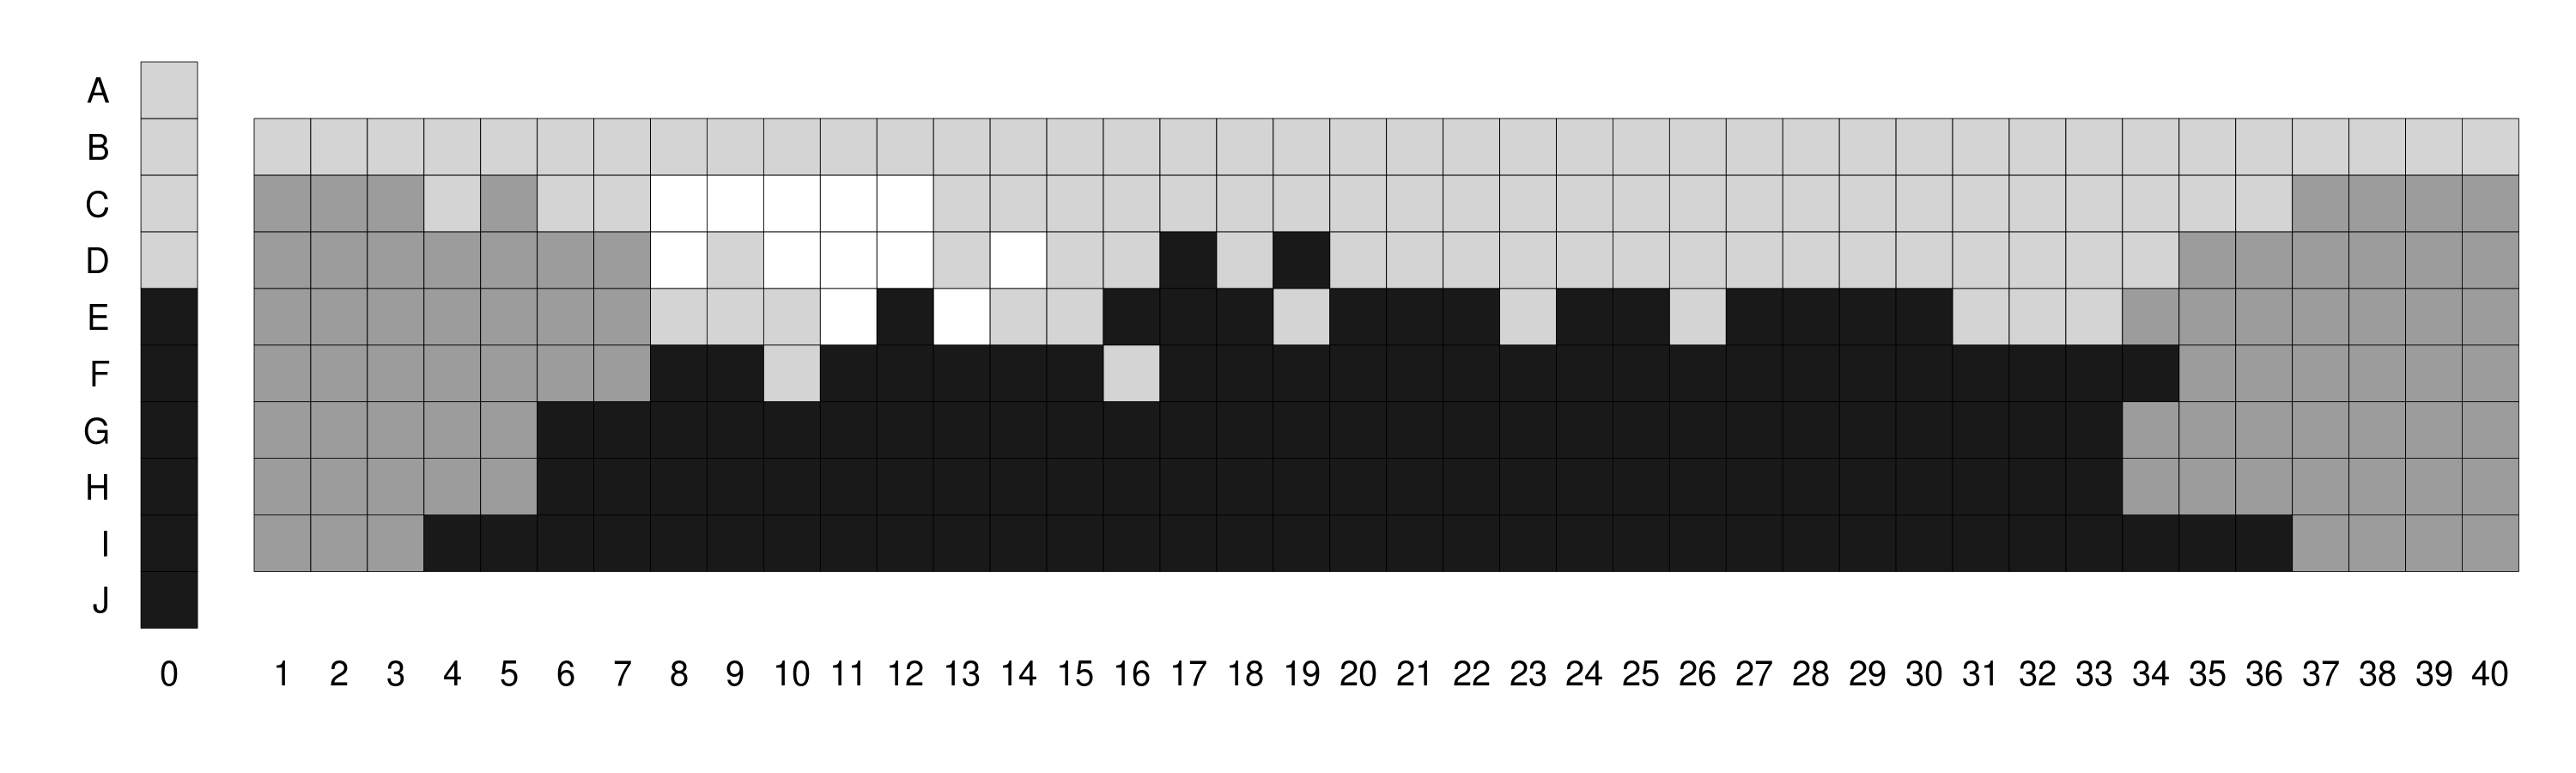
\includegraphics[width=0.48\columnwidth]{Kwerba}

\label{fig:kwerba}

}\hfill{}\subfloat[Ch�cobo language. Average within-category accuracy: 0.690. Match with
simulation in Figure~\ref{fig:worst-simulation}: 0.524.]{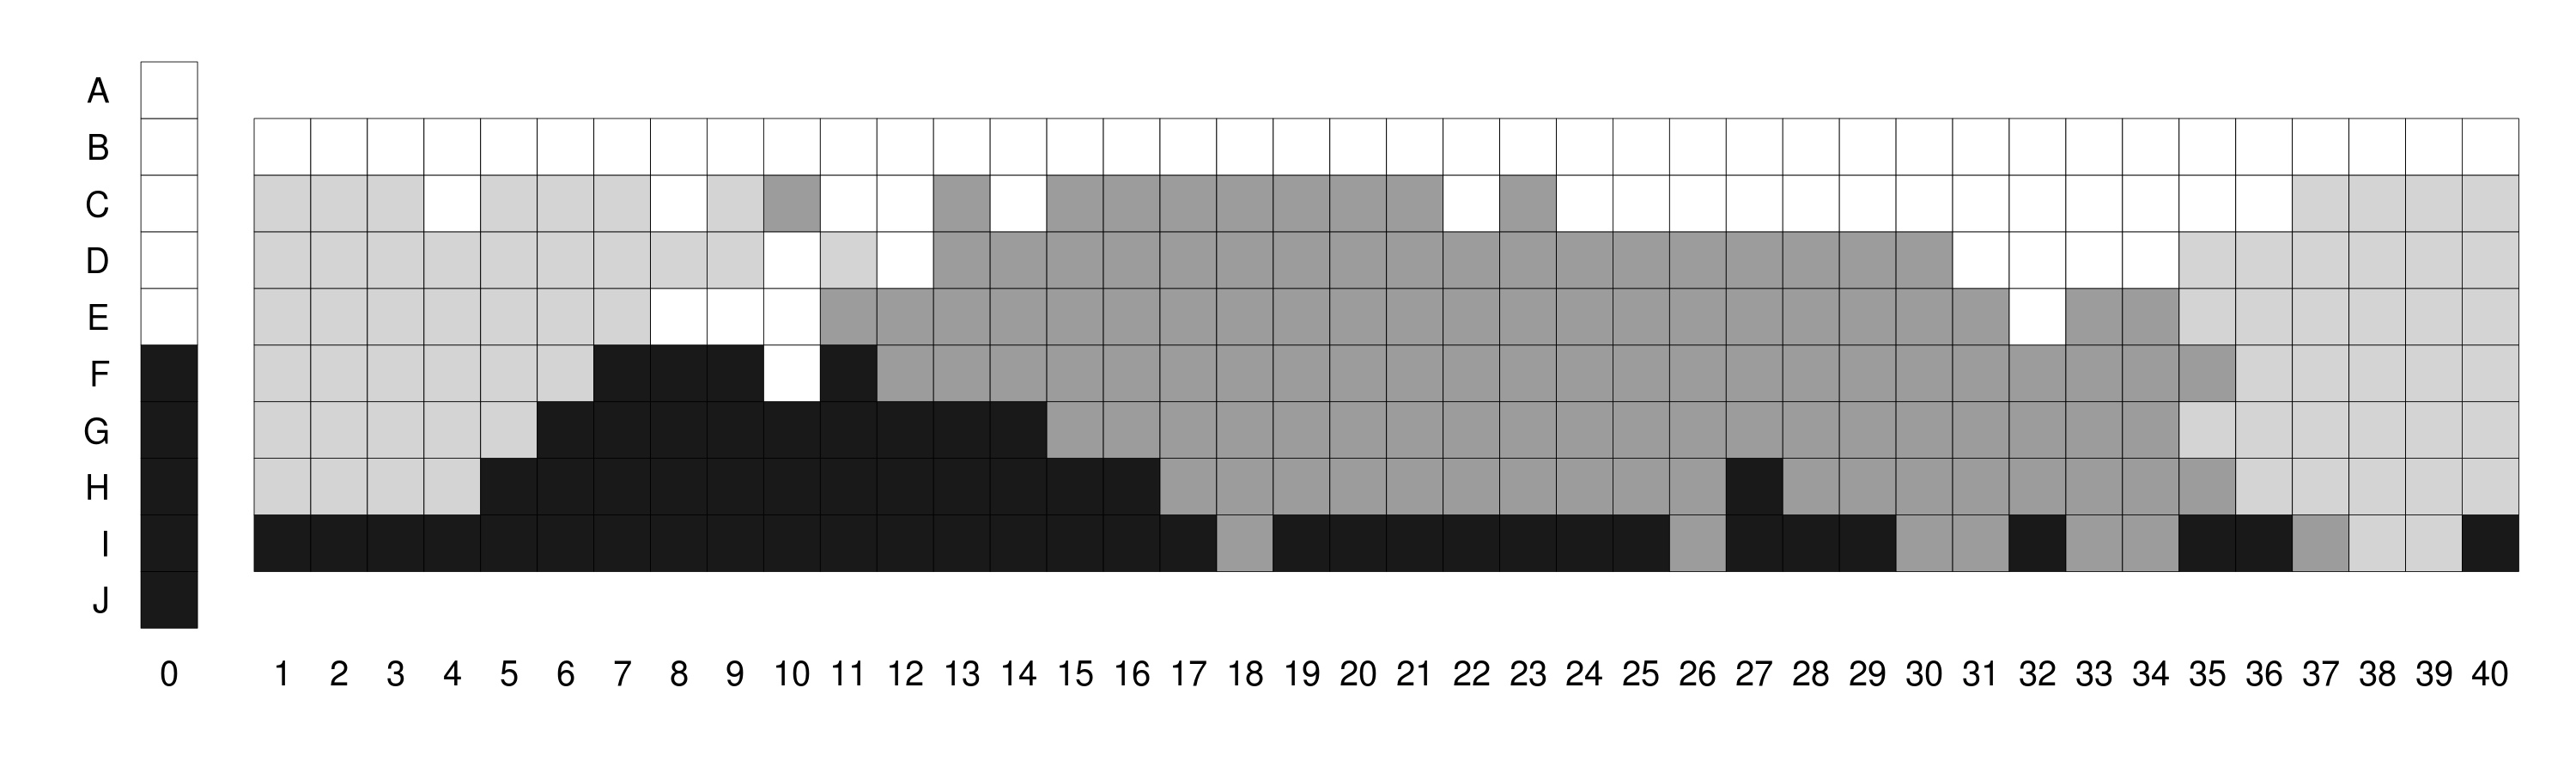
\includegraphics[width=0.48\columnwidth]{Chacobo}

\label{fig:chacobo}

}

\subfloat[Nafaanra language. Average within-category accuracy: 0.870. Match
with simulation in Figure~\ref{fig:best-simulation}: 0.658. Match
with Kwerba (Figure~\ref{fig:kwerba}): 0.779.]{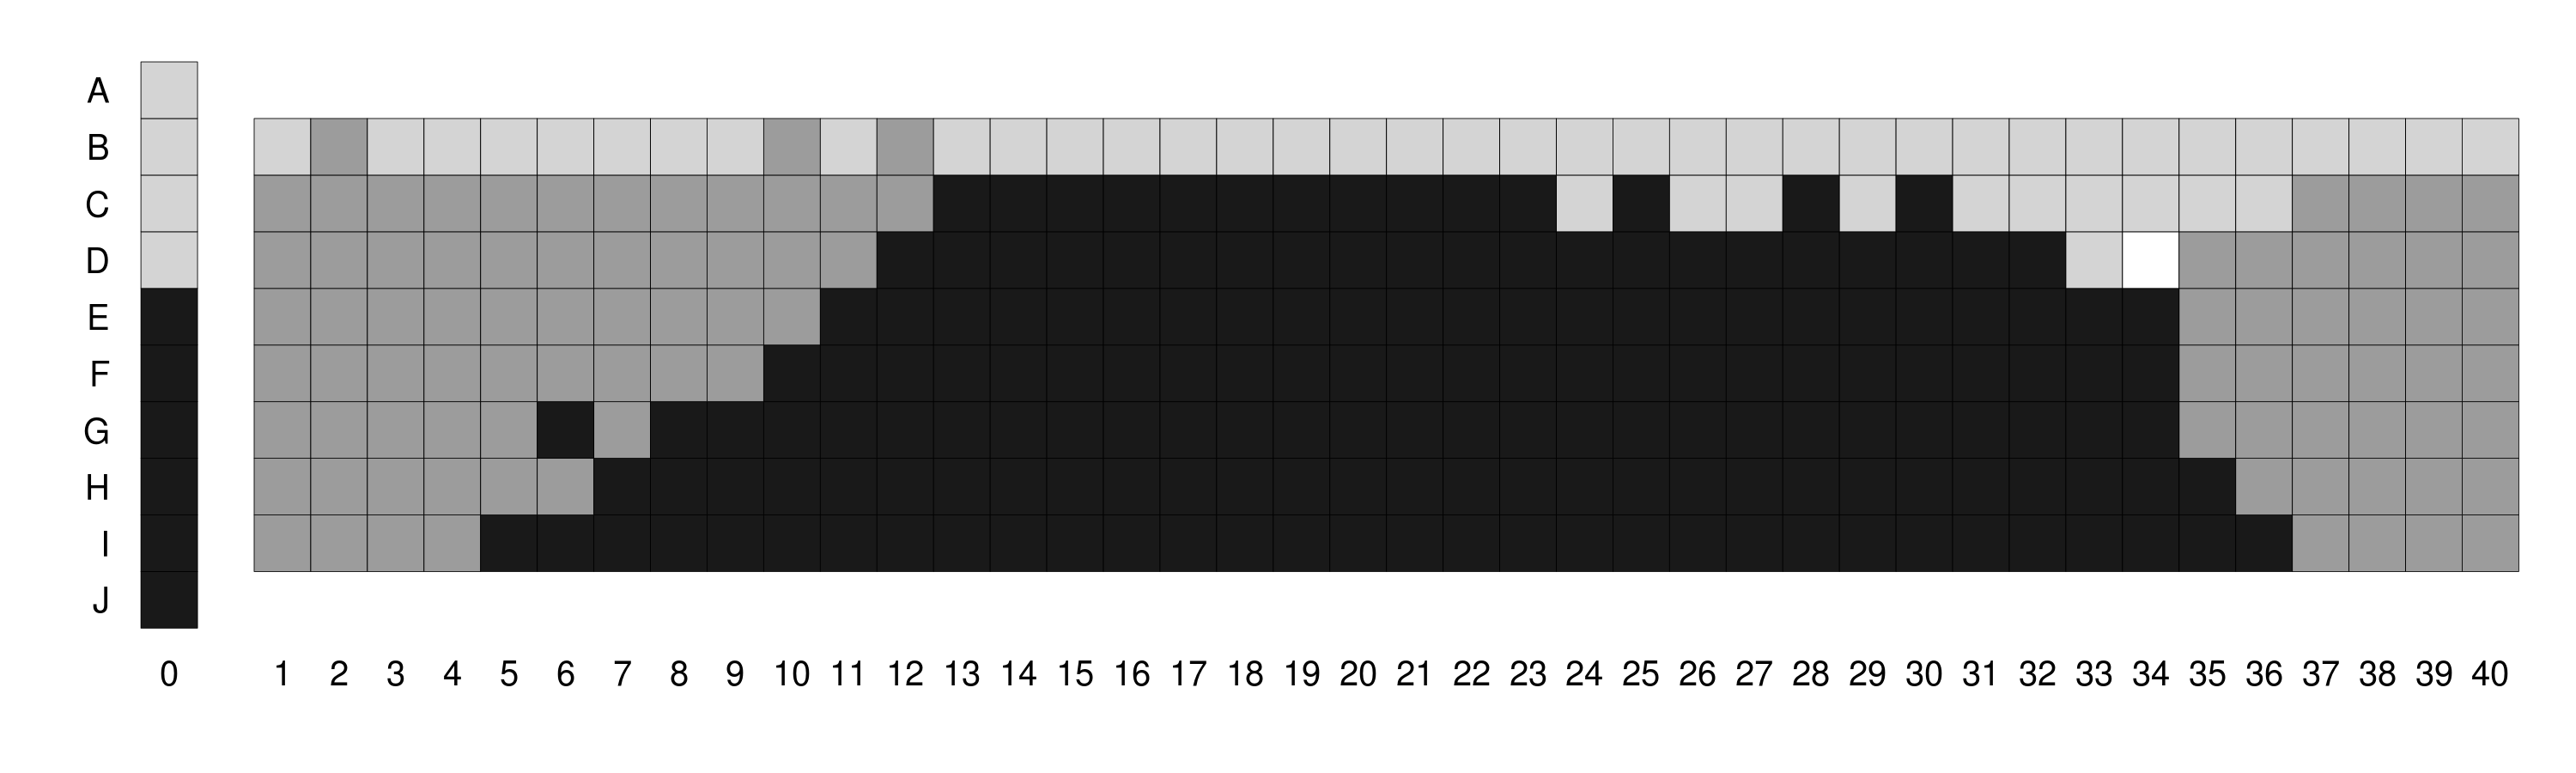
\includegraphics[width=0.48\columnwidth]{Nafaanra}

\label{fig:nafaanra}

}\hfill{}\subfloat[Culina language. Average within-category accuracy: 0.595. Match with
simulation in Figure~\ref{fig:worst-simulation}: 0.324. Match with
Ch�cobo (Figure~\ref{fig:chacobo}): 0.564.]{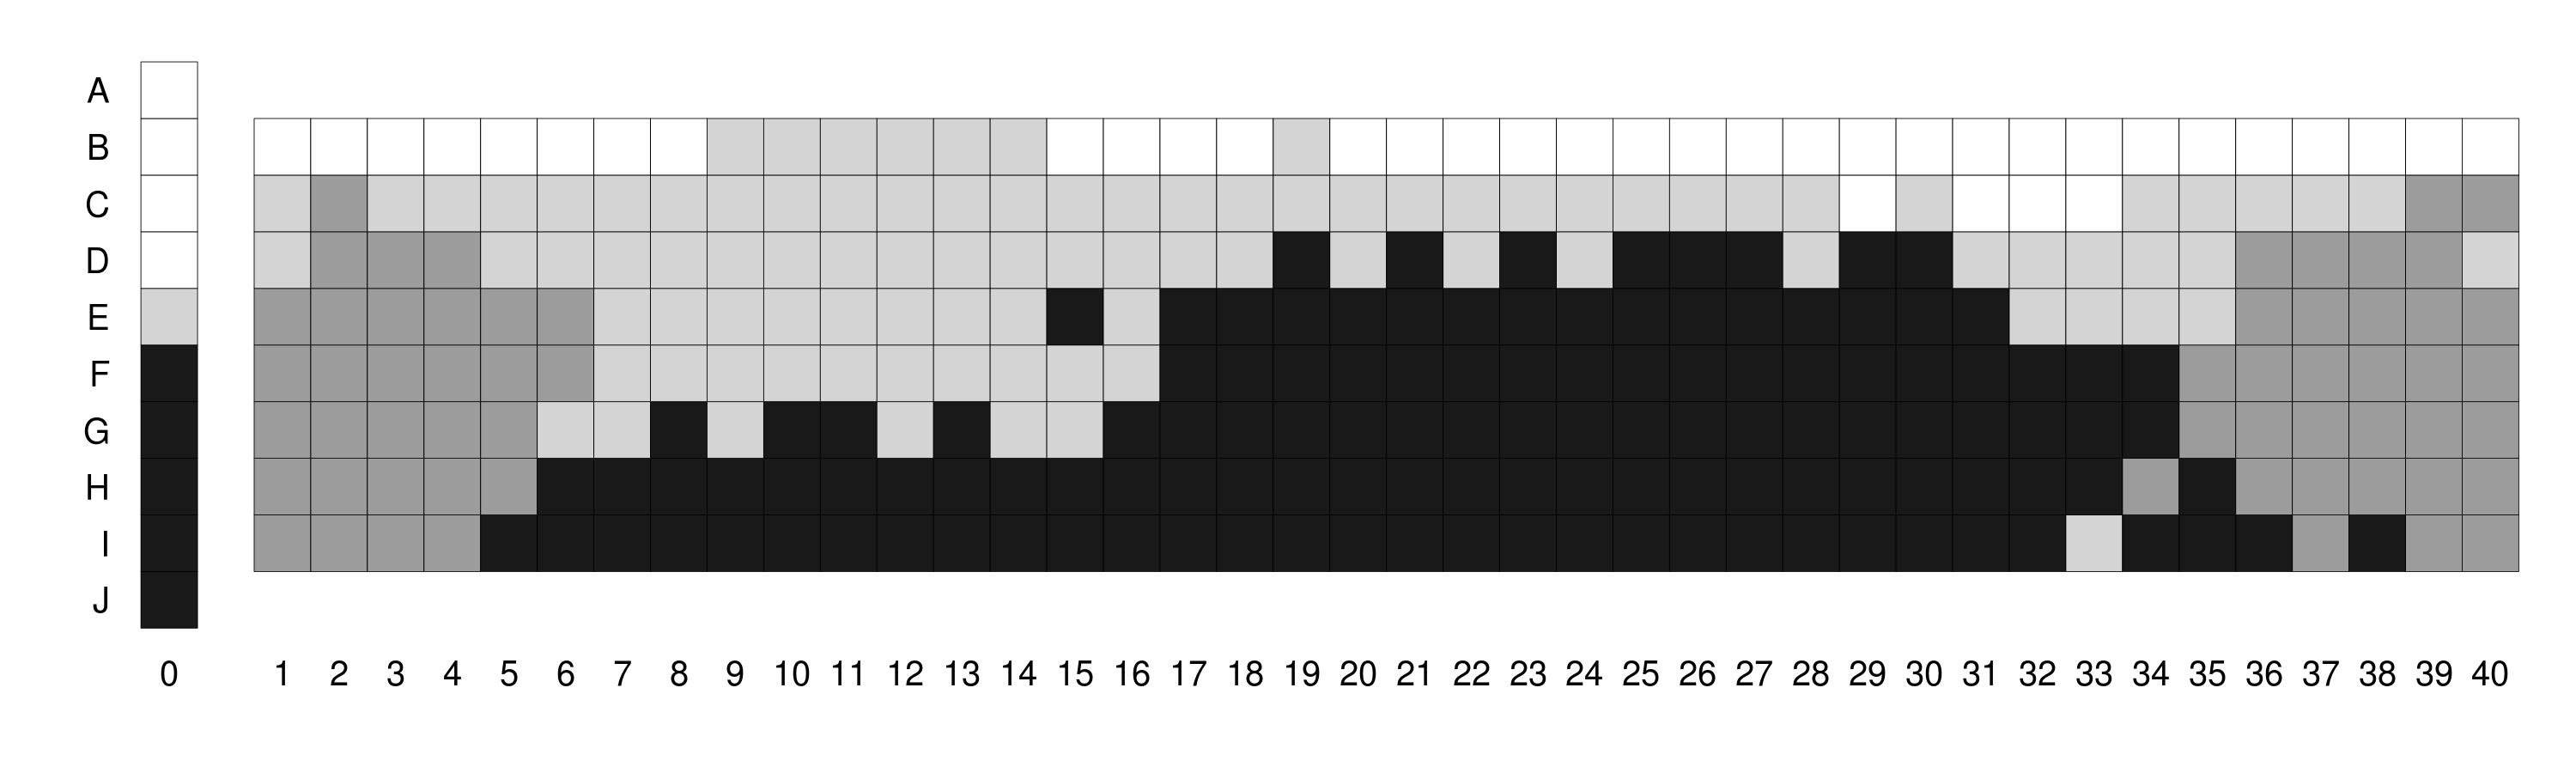
\includegraphics[width=0.48\columnwidth]{Culina}

\label{fig:culina}

}

\caption{Simulation results and matches with WCS languages. Different shades of grey within a certain mode map correspond to different color terms but be aware that the same shades accross different mode maps are \emph{not} necessarily matched to each other.}


\label{fig:plots} 
\end{figure}


What the numbers indicate is that the simulations are approximating
the phenomenon, although in a limited way. As expected, the accuracy
values obtained by the simulation results are significantly higher
than those obtained by random assignment. However, they are also significantly
lower than the within-category accuracy values obtained by the languages
in the WCS, albeit closer to this scenario than to the random one.
The comparison with the perfect sphere scenario shows how important
the topology of the color space is: the accuracy values for this scenario
are quite close to the ones obtained by the simulation results. However,
they are also consistently lower, which indicates that our simulation
setup is capturing some other non-trivial characteristics of the phenomenon.

Unfortunately, due to time limitations, we were not able to perform
a more in-depth analysis of all the results. This is important future
work to identify weaknesses in the model and therefore explore improvements
to it. For example, we noticed that the distribution of the accuracy
values of the simulations for $n=3$ is actually bi-modal: 5 simulations
have accuracy values ranging from $0.394$ to $0.615$, with an average
of $0.474$, whereas the other 5 have accuracy values ranging from
$0.588$ to $0.788$, with an average of $0.691$. This indicates
that a large number of populations are getting stuck in some local
minimum and thus adding for example mutation and/or invention to the
model might give a big boost in overall performance.


\section{Discussion}

\label{sec:discussion}

Although we were not able to account for particular universals of
color categorization in line with Kay and Maffi~\cite{Kay99}, the
overall quantitative evaluation of the model is encouraging, especially
if you consider the best-case values achieved. We have shown that
a very simple similarity-maximization signaling game based on a realistic
color space can already approximate, even if slightly, real-world
basic color term usage. Furthermore, our result is in certain sense complementary to that of Regier et al.~\cite{Reg07}. Whereas their work establishes the inclination of the WCS categorical systems to optimality, taking the projection of the Munsell chips into the CIELAB space for granted, our model confirms that there is indeed a degree of realism in choosing just this projection to be partitioned. We would now like to discuss a number of limitations
of the model where there is room for improvement by future research.

First, we have largely neglected empiricist views on the nature of
categories, emphasizing the dependence of these on the character of
the empirical input of any individual. We did so in assuming flat
probabilistic distribution over the perceptual space of 330 points.
Instead, a more realistic distribution could be used which would reflect
distribution of colors in natural sceneries. Purely empiricist strategies
of deriving color categories, based on clustering of such realistically
distributed input, are assessed by Yendrikhovskij~\cite{Yendr01}
and Steels and Belpaeme~\cite{Steels05}. The latter show that realistic
distribution helps a population of agents to converge in their categorical
repertoires, but is not a sufficiently strong factor to establish
a full agreement. In our model, convergence is reached via linguistic
interaction anyway, and realistic color distribution might increase
the performance.

This suggestion, though, embodies a rather crude version of empiricism.
It would be even more desirable to integrate in the model ecological
significances of various colors found in the environment, which need
not correspond to overall representation of these colors in one's
visual field. For instance, it seems plausible that red, the color
of blood and of many ripe fruits, is a more important color to be
linguistically distinguished than, say, purple or turquoise, or even
blue of clear sky and green of vegetation. If grounded in independent
evidence, rather than mere speculation, this could be represented
in our model by a utility function differentiated over the perceptual
space.

Second, our model is clearly unrealistic in that it lets fixed numbers
of terms compete in the perceptual space equally from a random start.
Instead, we should let terms break into the space already partitioned
by previous ones, as is apparently the case in language evolution.
This might lead to categorical systems quite different from what we
got in our setting. Allowing new signals to be invented is not unusual
in signaling games and besides being more realistic it can even help
achieving convergence faster and avoiding certain undesirable equilibria~\cite[chapter 10]{Skyrms2010}.

Third, for reasons of simplicity we used the set of Munsell chips
projected in the CIELAB color space as the perceptual space for the
game. However, what would be more realistic would be to use the continuous
CIELAB space and only for purposes of evaluation against the WCS map
the results back to the set of Munsell chips.


\section{Conclusion}

Our contribution is a model which transparently embodies a small amount
of explanatory principles, and a method of refined evaluation, which
can be repeated for future models of the same phenomenon. We did not
fully succeed in obtaining the results we expected, but we got some
promising indicators that the model is on the right track. We provided
a number of suggestions for improvements and we believe that, with
those in place, the model could provide a very realistic account of
how certain quasi-universal patterns of basic color term usage can
arise.

\bibliographystyle{plain}
\bibliography{bibl}

\end{document}
